\section{Introduction to quantum algorithmic approaches}\label{sec:quant}
In this section we will construct quantum algorithms for calculating the isotropic energy terms of GFN2-xTB\cite{bannwarth2019}: $E^\Gamma$ from equation \ref{eq:Gamma} and $E^\gamma$ from equation \ref{eq:gamma}.
We will showcase two very different approaches to doing a calculation as a building block of a larger circuit.


The conceptually simplest approach is to directly translate classical logic circuits to the quantum world using ancillary qubits to ensure reversibility.
Here most of the computation happens in the state, and the result is readable in the bits of the measurement output.
This approach has seen some development beyond this simple translation resulting in some very qubit efficient primitives for multiplication and addition in particular\cite{draper2000,perez2017}.
This approach will be applied to both the $E^\Gamma$ and $E^\gamma$ terms, and be referred to as Quantum Digital Arithmetic in this report. 


Our second approach is Quantum Amplitude Arithmetic\cite{wang2020}. 
In this approach we try to prepare the desired result not as a easily read measurement result, but as part of the amplitude of a state, which determines the probabilities. This is useful when we want to rank solutions for further processing or sampling of good candidates with high probability.
We will use this approach for the $E^\Gamma$ term to prepare a qubit in the state $w\ket{0}+\alpha\ket{0}$ where we can choose $\alpha$ to be proportional to the $E^\Gamma$ of the molecule.
Alternatively we can choose $\alpha$ to be proportional to $E^\Gamma-E^\Gamma_H$ where $E^\Gamma_H$ is the $E^\Gamma$ energy for some known high energy isomer.
This is not something we imagine being a common thing to want, however it is something which we want for the total energy. 
The issue that is solved by subtracting a known high energy is the following:
We want large relative differences between stable isomers and unstable ones. 
This is to ensure that if we run a superposition of isomers though the circuits required for the complete GFN2-xTB method we are able to efficiently sample the low energy isomers in the isomer space.
Say we know all the energies; if all the energies lie between -100 and -101 (units not important), which may make a large difference, the relative difference is not large.
If we subtract the energy of a known high energy isomer of say -100.1 we get much larger relative differences where the low energy isomers will have a much larger amplitude on 1, $\alpha$, than the high energy isomers. 


%The final algorithmic approach we will explore uses quantum singular value transformations\cite{gilyen2019}.
%In this approach the calculations are being carried out in the singular values of block encoded matrices. 
%We will use this approach to calculate the $E^{ETH}$ term, as it involves a lot of elementwise matrix multiplications. 
%This is well suited for this approach.


For both of these approaches we will assume that we have access to some intricately prepared states. 
We will not go into how the are prepared other than the fact that classically we can generate the approximate geometries for entire isomer spaces without any other information. 
As any classical computation in theory also can be applied to a quantum computer after modifications to make it reversible it is a possibility to prepare these states. 
A sketch of the preparation could be to generate all the IDs of the isomers, create a superposition and then run the algorithms for determining the geometry on this superposition of IDs. 

As a final note leading in to the implementations Quantum Amplitude Amplification is not to be confused with Quantum Amplitude Amplification, both shortened to QAA some times. 
We will be very explicit in which we are discussing in this thesis.
\subsection{Calculating $E^\Gamma$ using Quantum Digital Arithmetic}
The GFN2-xTB $E^\Gamma$ term has the following form\cite{bannwarth2021}
\begin{equation}
    E^\Gamma = \frac{1}{3}\sum_A\sum_{\mu\in A} (q_{A,\mu})^3\Gamma_{A,\mu},
\end{equation}
where $q_{A,\nu}=\sum_B\sum_{\nu\in B}P_{\mu\nu}S_{\mu\nu}$ is the Mulliken partial charge of shell $\mu$ associated with atom $A$. $P, S$ are the density and overlap matrices. $\Gamma_{A,\mu} = \Gamma_A K_\mu$ is just the product of an element specific constant and a shell specific constant, for our purposes the element is always carbon and the shell is either the first or second in GFN2 thus we have 2 numbers $\Gamma_{\text{Carbon},0(1)}$ henceforth referred to as $\varGamma_{0(1)}$. 

\vspace{\baselineskip}
\noindent
Let us first rewrite the inner expression a bit given our new definition and knowledge of the atoms we are working with. 
\begin{equation}
    \sum_{\mu\in A} (q_{A,\mu})^3\Gamma_{A,\mu} = \sum_{\mu \in \{0,1\}} (q_{A,\mu})^3\varGamma_{\mu}
\end{equation}

To implement this equation as a circuit we want to be able to add the terms in the inner expression to an accumulator. 
Thus we need a unitary which computes this function on a given state $\ket{\varGamma_\mu}_\Gamma\ket{q_{A,\mu}}_Q\ket{acc}_E \to \ket{\varGamma_\mu}_\Gamma\ket{q_{A,\mu}}_Q\ket{acc+(q_{A,\mu})^3\varGamma_{\mu}}_E$. The subscripts on the kets refer to the quantum register they represent. 
Consider having access to the following fused multiply add unitary $\ket{A}\ket{B}\ket{acc} \to \ket{A}\ket{B}\ket{acc+A*B}$, call it $\text{MADD}_{A,B,C}$. 
Let us to our initial $\Gamma, Q, E$ registers add two ancillary registers, $W_1,W_2$. 
We can now apply the following unitary 
\begin{equation}
    \resizebox{.9\hsize}{!}{${E_i^\Gamma}_{(\Gamma,Q,W_1,W_2,E)} = \text{MADD}^\dagger_{\Gamma,Q,W_1}\text{MADD}^\dagger_{Q,W_1,W_2}\text{MADD}_{Q,W_2,E}\text{MADD}_{Q,W_1,W_2}\text{MADD}_{\Gamma,Q,W_1}$}
    \label{EiG}
\end{equation}
\begin{figure}[H]
    \centering
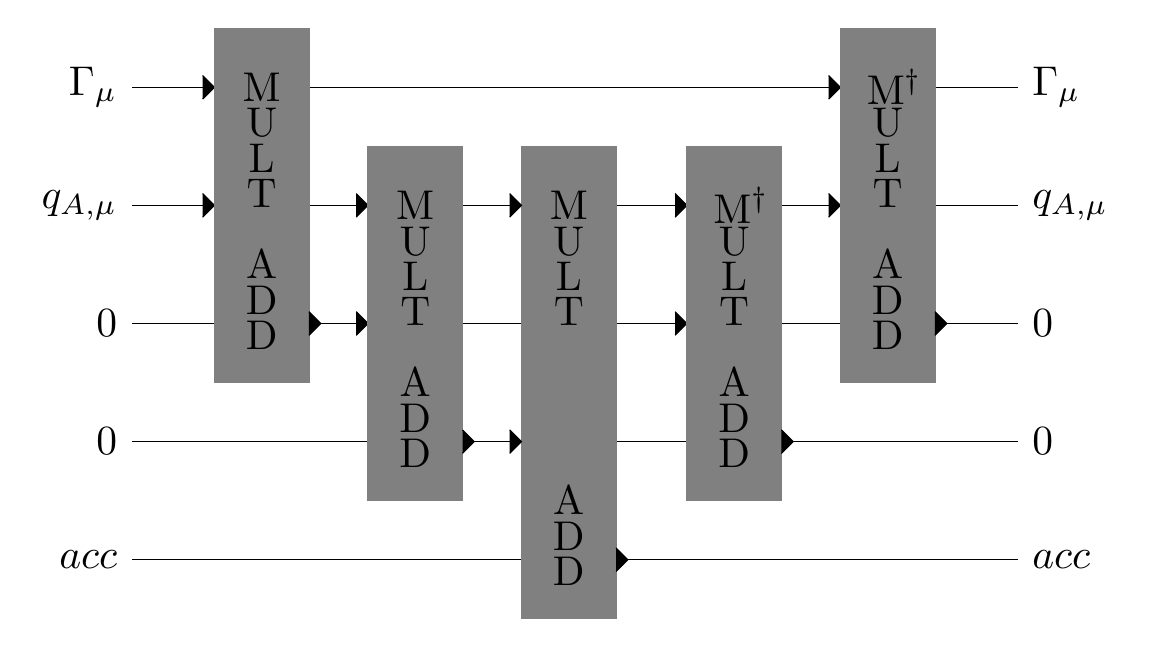
\begin{tikzpicture}[scale=1.5, transform shape]
    \node[rectangle,anchor=east] at (-1.5,4) {$\ket{\Gamma_\mu}$};
    \node[rectangle,anchor=east] at (-1.5,3) {$\ket{q_{A,\mu}}$};
    \node[rectangle,anchor=east] at (-1.5,2) {$\ket{0}$};
    \node[rectangle,anchor=east] at (-1.5,1) {$\ket{0}$};
    \node[rectangle,anchor=east] at (-1.5,0) {$\ket{acc}$};

    \node[rectangle,anchor=west] at ( 6,4) {$\ket{\Gamma_\mu}$};
    \node[rectangle,anchor=west] at ( 6,3) {$\ket{q_{A,\mu}}$};
    \node[rectangle,anchor=west] at ( 6,2) {$\ket{0}$};
    \node[rectangle,anchor=west] at ( 6,1) {$\ket{0}$};
    \node[rectangle,anchor=west] at ( 6,0) {$\ket{acc}$};
    \foreach \y in {0,...,4}
        \draw (-1.5,\y) -- (6,\y) ;
    \foreach \x in {0,...,1}{
        \filldraw[black] (\x*1.3-.9,2.9-\x) -- (\x*1.3-.8,3-\x) -- (\x*1.3-.9,3.1-\x);
        \filldraw[black] (\x*1.3-.9,3.9-\x) -- (\x*1.3-.8,4-\x) -- (\x*1.3-.9,4.1-\x);
        \filldraw[gray] (-0.8+\x*1.3+0,2-\x+2.5) rectangle (0+\x*1.3,1-\x+.5);
        \filldraw[black] (0+\x*1.3,1-\x+.9) -- (0+\x*1.3+0.1,1-\x+1) -- (0+\x*1.3,1-\x+1.1);
        \node[] at (-0.4+\x*1.3+0,2-\x+2.0) {M}; 
        \node[] at (-0.4+\x*1.3+0,2-\x+1.7) {U}; 
        \node[] at (-0.4+\x*1.3+0,2-\x+1.4) {L}; 
        \node[] at (-0.4+\x*1.3+0,2-\x+1.1) {T}; 
        \node[] at (-0.4+\x*1.3+0,2-\x+.5) {A}; 
        \node[] at (-0.4+\x*1.3+0,2-\x+.2) {D}; 
        \node[] at (-0.4+\x*1.3+0,2-\x-.1) {D}; 
    }
    \filldraw[gray] (-0.8+2*1.3+0,2-1+2.5) rectangle (0+2*1.3,1-2+.5);
    \filldraw[black] (0+2*1.3,1-2+.9) -- (0+2*1.3+0.1,1-2+1) -- (0+2*1.3,1-2+1.1);
MADD
    \filldraw[black] (2*1.3-.9,.9) -- (2*1.3-.8,1) -- (0+2*1.3-.9,1.1);
    \filldraw[black] (2*1.3-.9,2.9) -- (2*1.3-.8,3) -- (0+2*1.3-.9,3.1);
    \node[] at (-0.4+2*1.3+0,1+2.0) {M}; 
    \node[] at (-0.4+2*1.3+0,1+1.7) {U}; 
    \node[] at (-0.4+2*1.3+0,1+1.4) {L}; 
    \node[] at (-0.4+2*1.3+0,1+1.1) {T}; 
    \node[] at (-0.4+2*1.3+0,+.5) {A}; 
    \node[] at (-0.4+2*1.3+0,+.2) {D}; 
    \node[] at (-0.4+2*1.3+0,-.1) {D}; 
    \foreach \x in {0,...,1}{
        \filldraw[black] (4+\x*1.3-.9,2.9+\x) -- (4+\x*1.3-.8,3+\x) -- (4+\x*1.3-.9,3.1+\x);
        \filldraw[black] (4+\x*1.3-.9,1.9+\x) -- (4+\x*1.3-.8,2+\x) -- (4+\x*1.3-.9,2.1+\x);
        \filldraw[gray] (4+-0.8+\x*1.3+0,1+\x+2.5) rectangle (4+0+\x*1.3,+\x+.5);
        \filldraw[black] (4+0+\x*1.3,+\x+.9) -- (4+0+\x*1.3+0.1,+\x+1) -- (4+0+\x*1.3,+\x+1.1);
        \node[anchor=west] at (-0.4+\x*1.3+4-.3,1+\x+2.0) {M$ ^\dagger$}; 
        \node[] at (-0.4+\x*1.3+4,1+\x+1.7) {U}; 
        \node[] at (-0.4+\x*1.3+4,1+\x+1.4) {L}; 
        \node[] at (-0.4+\x*1.3+4,1+\x+1.1) {T}; 
        \node[] at (-0.4+\x*1.3+4,1+\x+.5) {A}; 
        \node[] at (-0.4+\x*1.3+4,1+\x+.2) {D}; 
        \node[] at (-0.4+\x*1.3+4,1+\x-.1) {D}; 
    }
\end{tikzpicture}
    \caption{Visualization of the circuit presented in equation \ref{EiG}. The arrows going into a block symbolise that qubit being used for the calculation happening in a given block. The arrows leaving a block symbolise the block changing something about that qubit. $\dagger$ is the complex conjugate used for doing an operation in reverse.}
\end{figure}
Let us follow the process:

\begin{align}
    &{E_i^\Gamma}_{(\Gamma,Q,W_1,W_2,E)}\ket{\varGamma_\mu}_\Gamma\ket{q_{A,\mu}}_Q\ket{0}_{W_1}\ket{0}_{W_2}\ket{acc}_E\\
    =&\resizebox{.9\hsize}{!}{$\text{MADD}^\dagger_{\Gamma,Q,W_1}\text{MADD}^\dagger_{Q,W_1,W_2}\text{MADD}_{Q,W_2,E}\text{MADD}_{Q,W_1,W_2}\ket{\varGamma_\mu}_\Gamma\ket{q_{A,\mu}}_Q\ket{\varGamma_\mu q_{A,\mu}}_{W_1}\ket{0}_{W_2}\ket{acc}_E$}\\
    =&\resizebox{.9\hsize}{!}{$\text{MADD}^\dagger_{\Gamma,Q,W_1}\text{MADD}^\dagger_{Q,W_1,W_2}\text{MADD}_{Q,W_2,E}\ket{\varGamma_\mu}_\Gamma\ket{q_{A,\mu}}_Q\ket{\varGamma_\mu q_{A,\mu}}_{W_1}\ket{\varGamma_\mu (q_{A,\mu})^2}_{W_2}\ket{acc}_E$}\\
    =&\resizebox{.9\hsize}{!}{$\text{MADD}^\dagger_{\Gamma,Q,W_1}\text{MADD}^\dagger_{Q,W_1,W_2}\ket{\varGamma_\mu}_\Gamma\ket{q_{A,\mu}}_Q\ket{\varGamma_\mu q_{A,\mu}}_{W_1}\ket{\varGamma_\mu (q_{A,\mu})^2}_{W_2}\ket{acc+\varGamma_\mu (q_{A,\mu})^3}_E\label{comp}$}\\
    =&\text{MADD}^\dagger_{\Gamma,Q,W_1}\ket{\varGamma_\mu}_\Gamma\ket{q_{A,\mu}}_Q\ket{\varGamma_\mu q_{A,\mu}}_{W_1}\ket{0}_{W_2}\ket{acc+\varGamma_\mu (q_{A,\mu})^3}_E\\
    =&\ket{\varGamma_\mu}_\Gamma\ket{q_{A,\mu}}_Q\ket{0}_{W_1}\ket{0}_{W_2}\ket{acc+\varGamma_\mu (q_{A,\mu})^3}_E\\
\end{align}
We see that already in eq. \ref{comp} we have the result we want in the accumulation register. We continue with the uncomputation of the $W_1,W_2$ registers purely to be able to reuse them in the remaining calculations. This saves the qubits required for having 2 ancillary registers for every calculation. The 'fused multiply add' gates here could be implementing using QFT multipliers\cite{perez2017} in which case we wouldn't need any ancillaries beyond the two mentioned. If we decompose our QFT multiplier into its components it is essentially a chain of QFT additions\cite{draper2000,perez2017} and multiplications by a constant power of two. These additions are built up of two components: (inverse) Fourier transforms and conditional rotations. When we chain them together like this however many of the transforms can be taken out as they are always followed or preceded by their inverse except for in the beginning and end. 



Let us say we are given a circuit, SDA, for encoding a molecule from its ID in the following manner, and a circuit $\text{DA}=\prod_{A}\prod_{\mu\in \{0,1\}} {E_i^\Gamma}_{(\Gamma_\mu,Q_{A,\mu},W_1,W_2,E)}$. Then 
\begin{equation}
\begin{split}
    \text{DA}\ \text{SDA}&\ket{id}_{ID}\ket{0}=\\
    \text{DA}&\ket{id}_{ID}\bigg(\bigotimes_{\mu\in \{0,1\}}\ket{\varGamma_\mu}_{\Gamma_\mu}\bigotimes_{A}\ket{q_{A,\mu}}_{Q_{A,\mu}}\bigg)\ket{0}_{W_1}\ket{0}_{W_2}\ket{0}_E =\\
    &\ket{id}_{ID}\bigg(\bigotimes_{\mu\in \{0,1\}}\ket{\varGamma_\mu}_{\Gamma_\mu}\bigotimes_{A}\ket{q_{A,\mu}}_{Q_{A,\mu}}\bigg)\ket{0}_{W_1}\ket{0}_{W_2}\ket{E^\Gamma_{id}}_E\\
\end{split}
\end{equation}
\noindent
will give us the $E^\Gamma$ energy term in the E register corresponding to the ID in the ID register.
Let us look at what happens as we are given a superposition of molecules as input instead. We will use a method introduced in the same paper\cite{wang2020} as Quantum Amplitude Arithmetic for sampling the low energy candidates. This will lead us gently into the later section where we use Quantum Amplitude Arithmetic to construct a circuit for calculating $E^\Gamma$.

\subsection{Sampling using Quantum Amplitude Arithmetic}
Assume that we are given an equal superposition of all the canonical IDs of the fullerenes in an isomer-space. We can apply SDA to set up the encoding and then apply $DA$. We now have computed the $E^\Gamma$ energies for every isomer. However we can only sample once.
Let us say that we are interested in the isomers with the lowest energies. We then would like the probability of sampling an isomer to be proportional to the gap between the highest energy and the energy of the isomer. 


\vspace{\baselineskip}
Wang et al. use their introduced addition and multiplication primitives to construct a probabilistic circuit which transforms the state $\ket{x}_D\ket{0}_C\ket{0}_W \to \big[\frac{1}{2}\frac{1}{2^n}\big]x\ket{x}_D\ket{0}_C\ket{1}_W+\alpha\ket{\omega}_{D \otimes C\otimes W}$ where $\alpha$ is some normalization factor, and $\ket{\omega}$ is some state with no overlap with the state containing all 0's in the control register, $C$, and 1 in the work register, $W$.
This property makes it very easy to check if the circuit succeeded, we can just use the measurement output that collapses the state to see if we measured the correct pattern of all zeroes and a one. The term in the brackets is the probability of success with $n$ being the number of bits used to describe $x$. $\alpha$ is then related to the probability of failure as the result should be normalised. 


\vspace{\baselineskip}
When using this circuit we can treat the $E$ register containing our resulting $E^\Gamma$ term as the data register, $D$. We can reuse the $W_1,W_2$ registers as the control and work registers. Let us take a look at that.
\begin{equation}
   \resizebox{.9\hsize}{!}{$\begin{split}
       \sum_{id\in \text{isomers}}&\ket{id}_{ID}\bigg(\bigotimes_{\mu\in \{0,1\}}\ket{\varGamma_\mu}_{\Gamma_\mu}\bigotimes_{A}\ket{q_{A,\mu}}_{Q_{A,\mu}}\bigg)\ket{0}_{W_1}\ket{0}_{W_2}\ket{E^\Gamma}_E =\\ 
       \sum_{id\in \text{isomers}}&\ket{id}_{ID}\bigg(\bigotimes_{\mu\in \{0,1\}}\ket{\varGamma_\mu}_{\Gamma_\mu}\bigotimes_{A}\ket{q_{A,\mu}}_{Q_{A,\mu}}\bigg)\left(\frac{1}{2}\frac{E^\Gamma_{id}}{2^n}\ket{0}_{W_1}\ket{1}_{W_2}\ket{E^\Gamma_{id}}_E+\alpha_{id}\ket{\omega_{id}}\right) \\ 
   \end{split}$}
\end{equation}
If we now sample from this superposition and postselect for $W_1 = 0$ and $W_2 = 1$ we are more likely to sample a low energy fullerene. The likelihood of sampling a given canonical fullerene ID is now proportional with $E^\Gamma_{id}$ for that fullerene.
Let us now look at what it would take to prepare the $E^\Gamma_{id}$ energies directly in the amplitude using Quantum Amplitude Arithmetic. 


\subsection{Calculating $E^\Gamma$ with Quantum Amplitude Arithmetic.}
In this section we will encode a molecule as follows
\begin{equation}
   \resizebox{.9\hsize}{!}{$\begin{split}
       \text{SAA}&\ket{id}_{ID}\ket{0}_{E,E_w,C_E,q_{o(1,2,3)},\Gamma_w,\Gamma_{1,\dots,n},q_{1,\dots,n},C_{1,\dots,\lceil log(n+1) \rceil}}\\
       =&\ket{id}_{ID}\ket{0}_{E,E_w,C_E,q_{o(1,2,3)},\Gamma_w}\bigotimes_{\mu\in\{0,1\}}\ket{\varGamma_\mu}_{\Gamma_{1,\dots,n}}\bigotimes_{A}\ket{q_{A,\mu}}_{q_{1,\dots,n}}\ket{0}_{C_{1,\dots,\lceil log(n+1) \rceil}}
   \end{split}$}
\end{equation}
Again we will not go into detail with the SAA circuit.

We now present a circuit for computing $E^\Gamma-E^\Gamma_H$ on a one atom molecule, with 4 bits of precision, with a single shell and therefore $\Gamma$ value. It is trivial to increase precision as it only involves straight forwards extension of the crimson region to use more qubits for $q,\ \Gamma$ and $C$.
\begin{figure}[H]
    \centering
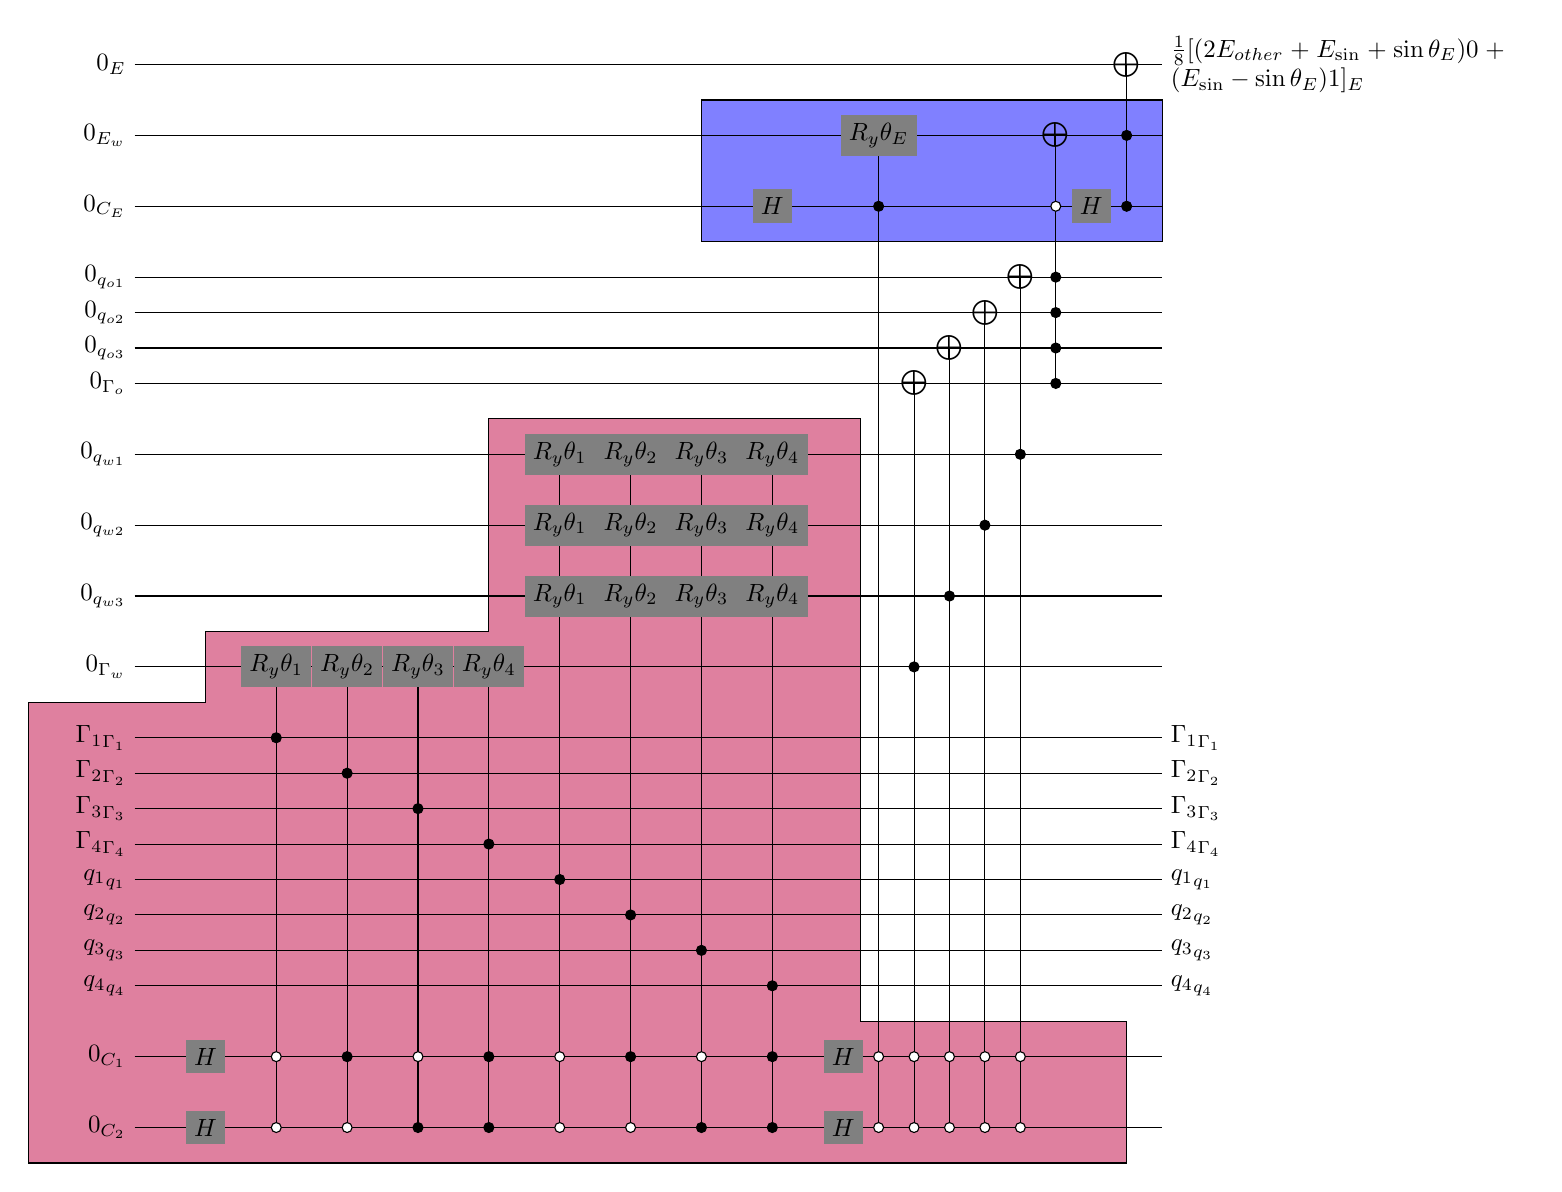
\begin{tikzpicture}[scale=0.9, transform shape]
    \draw[fill=purple!50] (-2.5,-.5) -- (-2.5,6) -- (0,6) -- (0,7) -- (4,7) -- (4,10) -- (9.25,10) -- (9.25,1.5) -- (13,1.5) -- (13,-.5) -- cycle;
    \draw[fill=blue!50] (7,12.5) -- (7,14.5) -- (13.5,14.5) -- (13.5,12.5) -- cycle;
    \foreach \y in {1,...,3}{
        \node[rectangle,anchor=east] at (-1,12.5-0.5*\y) {$\ket{0}_{q_{o\y}}$};
        \node[rectangle,anchor=east] at (-1,10.5-\y) { $\ket{0}_{q_{w\y}}$};
    }
    \node[rectangle,anchor=east] at (-1,10.5) {$\ket{0}_{\Gamma_o}$};
    \node[rectangle,anchor=east] at (-1,6.5) { $\ket{0}_{\Gamma_{w}}$};

    \node[text width=5cm,anchor=west] at (13.5,15) { $\frac{1}{8}[(2E_{other}+E_{\sin}+\sin\theta_E)\ket{0}+(E_{\sin}-\sin\theta_E)\ket{1}]_{E}$};


    \foreach \y in {1,...,4}
        \node[rectangle,anchor=east] at (-1,6-.5*\y) { $\ket{\Gamma_{\y}}_{\Gamma_{\y}}$};
    \foreach \y in {1,...,4}
        \node[rectangle,anchor=east] at (-1,4-.5*\y) { $\ket{q_{\y}}_{q_{\y}}$};
    \foreach \y in {1,2}
        \node[rectangle,anchor=east] at (-1,2-\y) { $\ket{0}_{C_{\y}}$};
    \node[rectangle,anchor=east] at (-1,13) { $\ket{0}_{C_E}$};
    \node[rectangle,anchor=east] at (-1,14) { $\ket{0}_{E_w}$};
    \node[rectangle,anchor=east] at (-1,15) { $\ket{0}_{E}$};

    \foreach \y in {1,...,4}
        \node[rectangle,anchor=west] at (13.5,6-.5*\y) { $\ket{\Gamma_{\y}}_{\Gamma_{\y}}$};
    \foreach \y in {1,...,4}
        \node[rectangle,anchor=west] at (13.5,4-.5*\y) { $\ket{q_{\y}}_{q_{\y}}$};

    \foreach \y in {0,...,2}
        \draw (-1,\y) -- (13.5,\y) ;
    \foreach \y in {3,...,9}
        \draw (-1,1+.5*\y) -- (13.5,1+.5*\y) ;
    \foreach \y in {1,...,3}
        \draw (-1,10.5+0.5*\y) -- (13.5,10.5+0.5*\y) ;
    \foreach \y in {1,...,3}
        \draw (-1,12+\y) -- (13.5,12+\y) ;
    \foreach \y in {10,...,14}
        \draw (-1,\y-3.5) -- (13.5,\y-3.5) ;
    \foreach \x in {1,...,4}{
        \draw (\x,0) -- (\x,6.5);
        \draw (\x+4,0) -- (\x+4,9.5);
    }
    \node[rectangle,fill=gray] at (0,0) {$H$} ;
    \node[rectangle,fill=gray] at (0,1) {$H$} ;
    \node[rectangle,fill=gray] at (9,0) {$H$} ;
    \node[rectangle,fill=gray] at (9,1) {$H$} ;
    \node[rectangle,fill=gray] at (8,13) {$H$} ;
    \node[rectangle,fill=gray] at (12.5,13) {$H$} ;
    \foreach \x in {1,...,4}{
        \node[rectangle,fill=gray] at (\x,6.5) {$R_y\theta_\x$} ;
        \foreach \y in {7.5,...,9.5}{
            \node[rectangle,fill=gray] at (\x+4,\y) {$R_y\theta_\x$} ;
        }
    }
    \draw (9.5,0) -- (9.5,14);
    \node[rectangle,fill=gray] at (9.5,14) {$R_y\theta_E$} ;
    \filldraw[black] (9.5,13) circle (2pt);
    \filldraw[white,draw=black] (9.5,0) circle (2pt);
    \filldraw[white,draw=black] (9.5,1) circle (2pt);

    \node[rectangle] at (12,14) {$\bigoplus$};
    \draw (12,10.5) -- (12,14);
    \foreach \y in {0,...,3}{
        \filldraw[black] (12,10.5+.5*\y) circle (2pt);
    }
    \filldraw[white,draw=black] (12,13) circle (2pt);
    \draw (13,13) -- (13,15);
    \node[rectangle] at (13,15) {$\bigoplus$};
    \filldraw[black] (13,13) circle (2pt);
    \filldraw[black] (13,14) circle (2pt);
    \foreach \a in {8,...,1}{
        \filldraw[black] (\a,6-0.5*\a) circle (2pt);
    }
    \foreach \g in {0,...,3}{
        \draw (10+0.5*\g,0) -- (10+0.5*\g,10.5+0.5*\g);
        \filldraw[white,draw=black] (10+0.5*\g,0) circle (2pt);
        \filldraw[white,draw=black] (10+0.5*\g,1) circle (2pt);
        \node[rectangle] at (0.5*\g+10,0.5*\g+10.5) {$\bigoplus$};
        \filldraw[black] (0.5*\g+10,\g+6.5) circle (2pt);
    }
    \foreach \x in {0,4}{
        \filldraw[black] (\x+2,1) circle (2pt);
        \filldraw[black] (\x+3,0) circle (2pt);
        \filldraw[black] (\x+4,1) circle (2pt);
        \filldraw[black] (\x+4,0) circle (2pt);
    }
    \foreach \x in {0,4}{
        \filldraw[white,draw=black] (\x+2,0) circle (2pt);
        \filldraw[white,draw=black] (\x+3,1) circle (2pt);
        \filldraw[white,draw=black] (\x+1,0) circle (2pt);
        \filldraw[white,draw=black] (\x+1,1) circle (2pt);
    }
\end{tikzpicture}
\caption{Circuit for computing $E^\Gamma-E^\Gamma_H$ on a one atom molecule where the charge $q$ and $\Gamma$ are described using 4 bites. The crimson shaded area scales with the number of bits. The blue shaded area is for subtracting $E^\Gamma_H$ and is completely optional.}
\end{figure}
This circuit is built from the addition and multiplication primitives introduced in the QA-Arithmetic paper\cite{wang2020}. We also do a slight modification to get subtraction. 

If using more than one atom and shells the additional $q$'s and $\Gamma$'s can be added below and the result added to the final $E_w$ register using an extra addition. $C_E$ should be scaled appropriately as the base 2 logarithm of the number of $q,\Gamma$ pairs plus 1.   

Let us go though the mathematics of our 4 bit example to show that A.) it is sound and B.) make the areas that will be extended more obvious. 

The controlled gate notation here is the following, $t$ is the target register and $c1,c2,c3,\dots$ are the control registers. $a,b,c,\dots$ are all $1$ except if there is a bar over the corresponding $c1,c2,c3,\dots$ in which case it is $0$. 
\begin{equation}
    \begin{split}
        CU^{c1,c2,c3,\dots}_t = (U_t-I_t)\otimes &\ket{a}\bra{a}_{c1} \otimes \ket{b}\bra{b}_{c2} \otimes \ket{c}\bra{c}_{c3}\otimes\dots+\\ 
        \sum_{\alpha,\beta,\zeta,\dots\in\{0,1\}}I_t\otimes &\ket{\alpha}\bra{\alpha}_{c1} \otimes \ket{\beta}\bra{\beta}_{c2} \otimes \ket{\zeta}\bra{\zeta}_{c3}\otimes\dots. 
    \end{split}
\end{equation}
As we do the calculation we neglect writing out the $q_{1,2,3,4},\Gamma_{1,2,3,4}$ as they never change throughout, we also neglect the registers outside of the crimson region for now. 
We begin by applying the Hadamard gates.
\begin{equation}
    \begin{split}
        H_{C1}H_{C2}&\ket{0000}_{q_{w(1,2,3)},\Gamma_w}\ket{ 00}_{C_{(1,2)}}=\\
        \frac{1}{2}(
        &\ket{0000}_{q_{w(1,2,3)},\Gamma_w}\ket{ 00}_{C_{(1,2)}}+\\
        &\ket{0000}_{q_{w(1,2,3)},\Gamma_w}\ket{ 01}_{C_{(1,2)}}+\\
        &\ket{0000}_{q_{w(1,2,3)},\Gamma_w}\ket{ 10}_{C_{(1,2)}}+\\
        &\ket{0000}_{q_{w(1,2,3)},\Gamma_w}\ket{ 11}_{C_{(1,2)}}
        )
    \end{split}
\end{equation}
When we apply the conditional rotation gates to a register such as $\Gamma_w$ we do the following
\begin{equation}
   \resizebox{.9\hsize}{!}{$\begin{split}
        CRy_{\Gamma_w}^{\Gamma_4,C_1,C_2}(2\theta_4)CRy_{\Gamma_w}^{\Gamma_3,\bar{C_1},C_2}(2\theta_3)CRy_{\Gamma_w}^{\Gamma_2,C_1,\bar{C_2}}(2\theta_2)&CRy_{\Gamma_w}^{\Gamma_1,\bar{C_1},\bar{C_2}}(2\theta_1)\\
        \frac{1}{2}\sum_{x_1,x_2\in\{0,1\}}\ket{0000}_{q_{w(1,2,3)},\Gamma_w}&\ket{ x_1x_2}_{C_{(1,2)}}=\\
        \frac{1}{2}(
        CRy_{\Gamma_w}^{\Gamma_1}(2\theta_1)\ket{0000}_{q_{w(1,2,3)},\Gamma_w}&\ket{ 00}_{C_{(1,2)}}+\\
        CRy_{\Gamma_w}^{\Gamma_2}(2\theta_2)\ket{0000}_{q_{w(1,2,3)},\Gamma_w}&\ket{ 01}_{C_{(1,2)}}+\\
        CRy_{\Gamma_w}^{\Gamma_3}(2\theta_3)\ket{0000}_{q_{w(1,2,3)},\Gamma_w}&\ket{ 10}_{C_{(1,2)}}+\\
        CRy_{\Gamma_w}^{\Gamma_4}(2\theta_4)\ket{0000}_{q_{w(1,2,3)},\Gamma_w}&\ket{ 11}_{C_{(1,2)}})=\\
        \frac{1}{2}(
        \ket{000}[\Gamma1(\cos\theta_1\ket{0}+\sin\theta_1\ket{1})+(1-\Gamma_1)\ket{0}]_{q_{w(1,2,3)},\Gamma_w}&\ket{ 00}+\\
        \ket{000}[\Gamma2(\cos\theta_2\ket{0}+\sin\theta_2\ket{1})+(1-\Gamma_2)\ket{0}]_{q_{w(1,2,3)},\Gamma_w}&\ket{ 01}+\\
        \ket{000}[\Gamma3(\cos\theta_3\ket{0}+\sin\theta_3\ket{1})+(1-\Gamma_3)\ket{0}]_{q_{w(1,2,3)},\Gamma_w}&\ket{ 10}+\\
        \ket{000}[\Gamma4(\cos\theta_4\ket{0}+\sin\theta_4\ket{1})+(1-\Gamma_4)\ket{0}]_{q_{w(1,2,3)},\Gamma_w}&\ket{ 11}
        )
   \end{split}$}
\end{equation}
To make our computations fit more easily on the page let us adopt the notation $\ket{\Psi^t_i}=t(\cos\theta_i\ket{0}+\sin\theta_i\ket{1})+(1-t)\ket{0}$ before redoing the application using our new notation. We also apply the rotation gates for the $q_w$ registers:
\begin{equation}
   \resizebox{.9\hsize}{!}{$\begin{split}
        CRy_{\Gamma_w}^{\Gamma_4,C_1,C_2}(2\theta_4)CRy_{\Gamma_w}^{\Gamma_3,\bar{C_1},C_2}(2\theta_3)CRy_{\Gamma_w}^{\Gamma_2,C_1,\bar{C_2}}(2\theta_2)&CRy_{\Gamma_w}^{\Gamma_1,\bar{C_1},\bar{C_2}}(2\theta_1)\\
        CRy_{q_{w1}}^{q_4,C_1,C_2}(2\theta_4)CRy_{q_{w1}}^{q_3,\bar{C_1},C_2}(2\theta_3)CRy_{q_{w1}}^{q_2,C_1,\bar{C_2}}(2\theta_2)&CRy_{q_{w1}}^{q_1,\bar{C_1},\bar{C_2}}(2\theta_1)\\
        CRy_{q_{w2}}^{q_4,C_1,C_2}(2\theta_4)CRy_{q_{w2}}^{q_3,\bar{C_1},C_2}(2\theta_3)CRy_{q_{w2}}^{q_2,C_1,\bar{C_2}}(2\theta_2)&CRy_{q_{w2}}^{q_1,\bar{C_1},\bar{C_2}}(2\theta_1)\\
        CRy_{q_{w3}}^{q_4,C_1,C_2}(2\theta_4)CRy_{q_{w3}}^{q_3,\bar{C_1},C_2}(2\theta_3)CRy_{q_{w3}}^{q_2,C_1,\bar{C_2}}(2\theta_2)&CRy_{q_{w3}}^{q_1,\bar{C_1},\bar{C_2}}(2\theta_1)\\
        \frac{1}{2}\sum_{x_1,x_2\in\{0,1\}}\ket{0000}_{q_{w(1,2,3)},\Gamma_w}&\ket{ x_1x_2}=\\
        \frac{1}{2}(
        CRy_{q_{w1}}^{q_1}(2\theta_1)CRy_{q_{w2}}^{q_1}(2\theta_1)CRy_{q_{w3}}^{q_1}(2\theta_1) CRy_{\Gamma_w}^{\Gamma_1}(2\theta_1)&\ket{0000}_{q_{w(1,2,3)},\Gamma_w}\ket{ 00}+\\
        CRy_{q_{w1}}^{q_2}(2\theta_2)CRy_{q_{w2}}^{q_2}(2\theta_2)CRy_{q_{w3}}^{q_2}(2\theta_2) CRy_{\Gamma_w}^{\Gamma_2}(2\theta_2)&\ket{0000}_{q_{w(1,2,3)},\Gamma_w}\ket{ 01}+\\
        CRy_{q_{w1}}^{q_3}(2\theta_3)CRy_{q_{w2}}^{q_3}(2\theta_3)CRy_{q_{w3}}^{q_3}(2\theta_3) CRy_{\Gamma_w}^{\Gamma_3}(2\theta_3)&\ket{0000}_{q_{w(1,2,3)},\Gamma_w}\ket{ 10}+\\
        CRy_{q_{w1}}^{q_4}(2\theta_4)CRy_{q_{w2}}^{q_4}(2\theta_4)CRy_{q_{w3}}^{q_4}(2\theta_4) CRy_{\Gamma_w}^{\Gamma_4}(2\theta_4)&\ket{0000}_{q_{w(1,2,3)},\Gamma_w}\ket{ 11})=\\
        \frac{1}{2}(
        \ket{\Psi^{q_1}_1\Psi^{q_1}_1\Psi^{q_1}_1\Psi^{\Gamma_1}_1}_{q_{w(1,2,3)},\Gamma_w}&\ket{ 00}+\\
        \ket{\Psi^{q_2}_2\Psi^{q_2}_2\Psi^{q_2}_2\Psi^{\Gamma_2}_2}_{q_{w(1,2,3)},\Gamma_w}&\ket{ 01}+\\
        \ket{\Psi^{q_3}_3\Psi^{q_3}_3\Psi^{q_3}_3\Psi^{\Gamma_3}_3}_{q_{w(1,2,3)},\Gamma_w}&\ket{ 10}+\\
        \ket{\Psi^{q_4}_4\Psi^{q_4}_4\Psi^{q_4}_4\Psi^{\Gamma_4}_4}_{q_{w(1,2,3)},\Gamma_w}&\ket{ 11}
        )
   \end{split}$}
\end{equation}
Let us now apply the second set of Hadamard gates:
\begin{equation}
   \resizebox{.9\hsize}{!}{$\begin{split}
        H_{C_1}H_{C_2}\frac{1}{2}(
        &\ket{\Psi^{q_1}_1\Psi^{q_1}_1\Psi^{q_1}_1\Psi^{\Gamma_1}_1 }\ket{00}+\\
        &\ket{\Psi^{q_2}_2\Psi^{q_2}_2\Psi^{q_2}_2\Psi^{\Gamma_2}_2 }\ket{01}+\\
        &\ket{\Psi^{q_3}_3\Psi^{q_3}_3\Psi^{q_3}_3\Psi^{\Gamma_3}_3 }\ket{10}+\\
        &\ket{\Psi^{q_4}_4\Psi^{q_4}_4\Psi^{q_4}_4\Psi^{\Gamma_4}_4 }\ket{11}
        )=\\
        \frac{1}{4}(
            &\ket{\Psi^{q_1}_1\Psi^{q_1}_1\Psi^{q_1}_1\Psi^{\Gamma_1}_1 }[\ket{00}+
            \ket{01}+
            \ket{10}+
            \ket{11}]+\\
            &\ket{\Psi^{q_2}_2\Psi^{q_2}_2\Psi^{q_2}_2\Psi^{\Gamma_2}_2 }[\ket{00}-
            \ket{01}+
            \ket{10}-
            \ket{11}]+\\
            &\ket{\Psi^{q_3}_3\Psi^{q_3}_3\Psi^{q_3}_3\Psi^{\Gamma_3}_3 }[\ket{00}+
            \ket{01}-
            \ket{10}-
            \ket{11}]+\\
            &\ket{\Psi^{q_4}_4\Psi^{q_4}_4\Psi^{q_4}_4\Psi^{\Gamma_4}_4 }[\ket{00}-
            \ket{01}-
            \ket{10}+
            \ket{11}]
    ) =\\ 
        \frac{1}{4}&\left[\ket{\Psi^{q_1}_1\Psi^{q_1}_1\Psi^{q_1}_1\Psi^{\Gamma_1}_1 }+\ket{\Psi^{q_2}_2\Psi^{q_2}_2\Psi^{q_2}_2\Psi^{\Gamma_2}_2 }+\ket{\Psi^{q_3}_3\Psi^{q_3}_3\Psi^{q_3}_3\Psi^{\Gamma_3}_3 }+\ket{\Psi^{q_4}_4\Psi^{q_4}_4\Psi^{q_4}_4\Psi^{\Gamma_4}_4 }\right]\ket{00}+\\
    \frac{1}{4}\bigg(&\left[\ket{\Psi^{q_1}_1\Psi^{q_1}_1\Psi^{q_1}_1\Psi^{\Gamma_1}_1 }-\ket{\Psi^{q_2}_2\Psi^{q_2}_2\Psi^{q_2}_2\Psi^{\Gamma_2}_2 }+\ket{\Psi^{q_3}_3\Psi^{q_3}_3\Psi^{q_3}_3\Psi^{\Gamma_3}_3 }-\ket{\Psi^{q_4}_4\Psi^{q_4}_4\Psi^{q_4}_4\Psi^{\Gamma_4}_4 }\right]\ket{01}+\\
        &\left[\ket{\Psi^{q_1}_1\Psi^{q_1}_1\Psi^{q_1}_1\Psi^{\Gamma_1}_1 }+\ket{\Psi^{q_2}_2\Psi^{q_2}_2\Psi^{q_2}_2\Psi^{\Gamma_2}_2 }-\ket{\Psi^{q_3}_3\Psi^{q_3}_3\Psi^{q_3}_3\Psi^{\Gamma_3}_3 }-\ket{\Psi^{q_4}_4\Psi^{q_4}_4\Psi^{q_4}_4\Psi^{\Gamma_4}_4 }\right]\ket{10}+\\
        &\left[\ket{\Psi^{q_1}_1\Psi^{q_1}_1\Psi^{q_1}_1\Psi^{\Gamma_1}_1 }-\ket{\Psi^{q_2}_2\Psi^{q_2}_2\Psi^{q_2}_2\Psi^{\Gamma_2}_2 }-\ket{\Psi^{q_3}_3\Psi^{q_3}_3\Psi^{q_3}_3\Psi^{\Gamma_3}_3 }+\ket{\Psi^{q_4}_4\Psi^{q_4}_4\Psi^{q_4}_4\Psi^{\Gamma_4}_4 }\right]\ket{11}
    \bigg) \\= 
        \frac{1}{4}&\left[\ket{\Psi^{q_1}_1\Psi^{q_1}_1\Psi^{q_1}_1\Psi^{\Gamma_1}_1 }+\ket{\Psi^{q_2}_2\Psi^{q_2}_2\Psi^{q_2}_2\Psi^{\Gamma_2}_2 }+\ket{\Psi^{q_3}_3\Psi^{q_3}_3\Psi^{q_3}_3\Psi^{\Gamma_3}_3 }+\ket{\Psi^{q_4}_4\Psi^{q_4}_4\Psi^{q_4}_4\Psi^{\Gamma_4}_4 }\right]\ket{00}+\ket{M}\\=&\ket{N}+\ket{M}
   \end{split}$}
\end{equation}
Before the next step let us define:
\begin{align}
    q_{\sin} =& q_1\sin\theta_1+q_2\sin\theta_2+q_3\sin\theta_3+q_4\sin\theta_4\\
    q_{other} =& q_1\cos\theta_1+q_2\cos\theta_2+q_3\cos\theta_3+q_4\cos\theta_4+4-q_1-q_2-q_3-q_4\\
    \Gamma_{\sin} =& \Gamma_1\sin\theta_1+\Gamma_2\sin\theta_2+\Gamma_3\sin\theta_3+\Gamma_4\sin\theta_4\\
    \Gamma_{other} =& \Gamma_1\cos\theta_1+\Gamma_2\cos\theta_2+\Gamma_3\cos\theta_3+\Gamma_4\cos\theta_4+4-\Gamma_1-\Gamma_2-\Gamma_3-\Gamma_4\\
    E_{\sin} =& \Gamma_{\sin}(q_{\sin})^3\\
    \begin{split}
        E_{other} = &\Gamma_{other}(q_{other}^3+3q_{other}^2q_{\sin}+3q_{other}q_{\sin}^2+q_{\sin}^3)\\
        &+\Gamma_{\sin}(q_{other}^3+3q_{other}^2q_{\sin}+3q_{other}q_{\sin}^2)
    \end{split}\\
    \ket{\sigma_t} = &t_{other}\ket{0}+t_{\sin}\ket{1}\\
\end{align}
Let us now add in the $ _o$ registers and apply the first 4 conditional not gates:
\begin{equation}
   \resizebox{.9\hsize}{!}{$\begin{split}
        CX_{q_{o1}}^{q_{w1},\bar{C_1},\bar{C_2}}CX_{q_{o2}}^{q_{w2},\bar{C_1},\bar{C_2}}CX_{q_{o3}}^{q_{w3},\bar{C_1},\bar{C_2}}CX_{\Gamma_o}^{\Gamma_w,\bar{C_1},\bar{C_2}}
        \ket{0000}_{E,q_{o(1,2,3)},\Gamma_o}&(\ket{N}+\ket{M})=\\
        \bigg(CX_{q_{o1}}^{q_{w1}}CX_{q_{o2}}^{q_{w2}}CX_{q_{o3}}^{q_{w3}}CX_{\Gamma_o}^{\Gamma_w}
        \ket{0000}\ket{N}\bigg)+\ket{0000}&\ket{M}=\\
        \ket{\sigma_q\sigma_q\sigma_q\sigma_\Gamma}_{q_{o(1,2,3)},\Gamma_{o}}\ket{N}+\ket{0000}&\ket{M}\\
   \end{split}$}
\end{equation}
Now let us disregard everything in the crimson region except the $C_1,C_2$ control registers and do the final gates involving the $ _o$ registers:
\begin{equation}
   \resizebox{.9\hsize}{!}{$\begin{split}
        H_{C_E}&CX_{E_w}^{\bar{C}_E,q_{o1},q_{o2},q_{o3},\Gamma_o}CRy_{E_w}^{C_E,\bar{C}_1,\bar{C}_2}(\theta_E)H_{C_E}\ket{000}_{E,E_w,C_E}
        \frac{1}{4}\bigg(
        \ket{\sigma_q\sigma_q\sigma_q\sigma_\Gamma}_{q_{o(1,2,3)},\Gamma_{o}}\ket{00}_{C_1,C_2}\\&+
        \ket{0000}_{q_{o(1,2,3)},\Gamma_o}[\ket{01}+\ket{10}+\ket{11}]_{C_1,C_2}\bigg)=\\
        H_{C_E}&\frac{1}{4}\bigg(\ket{0}\frac{1}{\sqrt{2}}\bigg[CX_{E_w}^{q_{o1},q_{o2},q_{o3},\Gamma_o}\ket{0}\ket{0}+Ry_{E_w}(\theta_E)\ket{0}\ket{1}\bigg]
        \ket{\sigma_q\sigma_q\sigma_q\sigma_\Gamma}_{q_{o(1,2,3)},\Gamma_{o}}\ket{00}_{C_1,C_2}\\&+
        \ket{00+0000}_{E,E_w,C_E,q_{o(1,2,3)},\Gamma_o}[\ket{01}+\ket{10}+\ket{11}]_{C_1,C_2}\bigg)=\\
        H_{C_E}&\frac{1}{4}\bigg(\ket{0}\frac{1}{\sqrt{2}}\bigg[\ket{\sigma_E}_{E_w}\ket{0}_{C_E}+(\cos\theta_E\ket{0}+\sin\theta_E\ket{1})_{E_w}\ket{1}_{C_E}\bigg]\ket{\sigma_q\sigma_q\sigma_q\sigma_\Gamma}_{q_{o(1,2,3)},\Gamma_{o}}\ket{00}_{C_1,C_2}\\&+
        \ket{00+0000}_{E,E_w,C_E,q_{o(1,2,3)},\Gamma_o}[\ket{01}+\ket{10}+\ket{11}]_{C_1,C_2}\bigg)=\\
        &\frac{1}{4}\bigg(\ket{0}\frac{1}{\sqrt{2}}\bigg[\ket{\sigma_E}_{E_w}\ket{+}_{C_E}+(\cos\theta_E\ket{0}+\sin\theta_E\ket{1})_{E_w}\ket{-}_{C_E}\bigg]\ket{\sigma_q\sigma_q\sigma_q\sigma_\Gamma}_{q_{o(1,2,3)},\Gamma_{o}}\ket{00}_{C_1,C_2}\\&+
        \ket{000000}_{E,E_w,C_E,q_{o(1,2,3)},\Gamma_o}[\ket{01}+\ket{10}+\ket{11}]_{C_1,C_2}\bigg)\\
   \end{split}$}
\end{equation}

\newpage
\noindent
Now we can neglect the $q_{o(1,2,3),\Gamma_o,C_1,C_2}$ registers too and do some preparatory manipulations before applying the final conditional not gate. 
\begin{equation}
   \resizebox{.9\hsize}{!}{$\begin{split}
        \frac{1}{4}\bigg(\ket{0}\frac{1}{\sqrt{2}}\bigg[&\ket{\sigma_E}_{E_w}\ket{+}_{C_E}+(\cos\theta_E\ket{0}+\sin\theta_E\ket{1})_{E_w}\ket{-}_{C_E}\bigg]+3\ket{000}\bigg)=\\
        \frac{1}{4}\bigg(\ket{0}\frac{1}{2}\bigg[&\ket{\sigma_E}_{E_w}\ket{0}_{C_E}+\ket{\sigma_E}_{E_w}\ket{1}_{C_E}+(\cos\theta_E\ket{0}+\sin\theta_E\ket{1})_{E_w}\ket{0}_{C_E}\\
        -(\cos\theta_E&\ket{0}+\sin\theta_E\ket{1})_{E_w}\ket{1}_{C_E}\bigg]+3\ket{000}\bigg)=\\
        \frac{1}{4}\bigg(
        \ket{0}\frac{1}{2}\bigg[&
        (\ket{\sigma_E}+\cos\theta_E\ket{0}+\sin\theta_E\ket{1})_{E_w}\ket{0}_{C_E}\\
        +&(\ket{\sigma_E}-\cos\theta_E\ket{0}-\sin\theta_E\ket{1})_{E_w}\ket{1}_{C_E}
        \bigg]+3\ket{000}\bigg)=\\
        \frac{1}{8}\bigg(
        \ket{0}&
        [\ket{\sigma_E}+\cos\theta_E\ket{0}+\sin\theta_E\ket{1}]_{E_w}\ket{0}_{C_E}\\
        +\ket{0}&[\ket{\sigma_E}-\cos\theta_E\ket{0}-\sin\theta_E\ket{1}]_{E_w}\ket{1}_{C_E}
        +6\ket{000}\bigg)=\\
        \frac{1}{8}\bigg(
         \ket{0}&[E_{other}\ket{0}+E_{\sin}\ket{1}+\cos\theta_E\ket{0}+\sin\theta_E\ket{1}]_{E_w}\ket{0}_{C_E}\\
        +\ket{0}&[E_{other}\ket{0}+E_{\sin}\ket{1}-\cos\theta_E\ket{0}-\sin\theta_E\ket{1}]_{E_w}\ket{1}_{C_E}
        +6\ket{000}\bigg)=\\
        \frac{1}{8}\bigg(
        \ket{0}&[(E_{other}+\cos\theta_E)\ket{0}+(E_{\sin}+\sin\theta_E)\ket{1}]_{E_w}\ket{0}_{C_E}\\
        +\ket{0}&[(E_{other}-\cos\theta_E)\ket{0}+(E_{\sin}-\sin\theta_E)\ket{1}]_{E_w}\ket{1}_{C_E}
        +6\ket{000}\bigg)=\\
        \frac{1}{8}\bigg(
        &(E_{other}+\cos\theta_E)\ket{000}+(E_{\sin}+\sin\theta_E)\ket{010}\\+
        &(E_{other}-\cos\theta_E)\ket{001}+(E_{\sin}-\sin\theta_E)\ket{011}+6\ket{000}\bigg)\\
   \end{split}$}
\end{equation}

\noindent
In the last step we just did, see that we can 'select' either addition or subtraction of $\sin\theta_E$ just by controlling our next gate on 010 or 011. 
We now apply the final conditional not gate:
\begin{equation}
   \resizebox{.9\hsize}{!}{$\begin{split}
        CX_{E}^{E_w,C_E}\frac{1}{8}\bigg(
        &(E_{other}+\cos\theta_E)\ket{000}+(E_{\sin}+\sin\theta_E)\ket{010}\\+
        &(E_{other}-\cos\theta_E)\ket{001}+(E_{\sin}-\sin\theta_E)\ket{011}+6\ket{000}\bigg)=\\
        \frac{1}{8}\bigg(
        &(E_{other}+\cos\theta_E)\ket{000}+(E_{\sin}+\sin\theta_E)\ket{010}\\+
        &(E_{other}-\cos\theta_E)\ket{001}+X_{E}(E_{\sin}-\sin\theta_E)\ket{011}+6\ket{000}\bigg)=\\
        \frac{1}{8}\bigg(
        &(E_{other}+\cos\theta_E)\ket{000}+(E_{\sin}+\sin\theta_E)\ket{010}\\+
        &(E_{other}-\cos\theta_E)\ket{001}+(E_{\sin}-\sin\theta_E)\ket{111}+6\ket{000}\bigg)\\
   \end{split}$}
\end{equation}
After applying those gates we see that the amplitude on $\ket{1}_{E}$ across the whole state is 
\begin{equation*}
   \resizebox{.9\hsize}{!}{$\frac{1}{8}(E_{\sin}-\sin\theta_E)=(\Gamma_1\sin\theta_1+\Gamma_2\sin\theta_2+\Gamma_3\sin\theta_3+\Gamma_4\sin\theta_4)(q_1\sin\theta_1+q_2\sin\theta_2+q_3\sin\theta_3+q_4\sin\theta_4)^3-\sin\theta_E.$}
\end{equation*}
Let us say we know the $E^\Gamma$ energy of some high energy molecule in the isomer space $$E^\Gamma_H = (0b0.\Gamma_H)(0b0.q_H)^3$$
If we specify 
$$\theta_i=arcsin\frac{1}{2^i},\quad\theta_E=arcsin[(0b0.\Gamma_H)(0b0.q_H)^3]$$ 
we get that $$E_{\sin}=(\frac{\Gamma_1}{2}+\frac{\Gamma_2}{2^2}+\frac{\Gamma_3}{2^3}+\frac{\Gamma_4}{2^8})(\frac{q_1}{2}+\frac{q_2}{2^2}+\frac{q_3}{2^3}+\frac{q_4}{2^8})^3=(0b0.\Gamma_1\Gamma_2\Gamma_3\Gamma_4)(0b0.q_1q_2q_3q_4)^3$$ and that $$\frac{1}{8}(E_{\sin}-\sin\theta_E)=\frac{1}{8}[(0b0.\Gamma_1\Gamma_2\Gamma_3\Gamma_4)(0b0.q_1q_2q_3q_4)^3-(0b0.\Gamma_H)(0b0.q_H)^3]$$. This is proportional to $E^\Gamma-E^\Gamma_H$ and thus the circuit is sound. 

We will now take a look at the $E^\gamma$ term.

\subsection{Calculating $E^\gamma$ using Quantum Digital Arithmetic}
The $E_\gamma$ term is formulated as follows:
\begin{gather}
    \eta_{AB,ll'} = \frac{1}{2}\left[\eta_A(1+K_A^l)+\eta_B(1+K_B^{l'})\right]\\
    R_{AB}^2 = (A_x-B_x)^2+(A_y-B_y)^2+(A_z-B_z)^2\\
    \gamma_{AB,ll'}=\frac{1}{\sqrt{R_{AB}^2+\eta_{AB,ll'}^{-2}}}\\
    E_\gamma=\frac{1}{2}\sum_{A,B}\sum_{l\in A}\sum_{l'\in B} q_lq_{l'}\gamma_{AB,ll'}\\
\end{gather}
For fullerenes we can view $\eta_{AB,ll'}^{-2}$ as only dependant on the angular momenta $l$ and $l'$, so there are 4 configurations as there are only 2 shells for carbon in GFN2-xTB and the rest of the terms are constants. Additionally $l=0,l'=1$ and $l=1,l'=0$ are equivalent. Thus we don't actually have to compute $\eta$ during the quantum circuit and can just bake in those 3 configurations as constants.  
A small circuit for calculating $R_{AB}^2$ could be made up of 3 repetitions of the $\text{DIFF}^2$ circuit described bellow which for 2 numbers $a,b$ and an accumulator $acc$ computes $acc + (a-b)^2$ :
\begin{figure}[H]
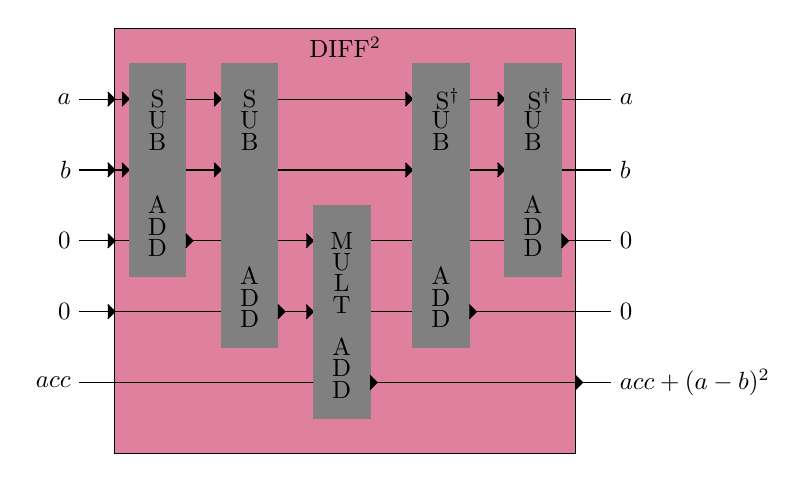
\begin{tikzpicture}[scale=.9, transform shape]
    \filldraw[fill=purple!50] (-1,5) rectangle (5.5,-1) ;
    \node[anchor=north] at (2.25,5) {DIFF$ ^2$};
    \node[rectangle,anchor=east] at (-1.5,4) {$\ket{a}$};
    \node[rectangle,anchor=east] at (-1.5,3) {$\ket{b}$};
    \node[rectangle,anchor=east] at (-1.5,2) {$\ket{0}$};
    \node[rectangle,anchor=east] at (-1.5,1) {$\ket{0}$};
    \node[rectangle,anchor=east] at (-1.5,0) {$\ket{acc}$};

    \node[rectangle,anchor=west] at (6,4) {$\ket{a}$};
    \node[rectangle,anchor=west] at (6,3) {$\ket{b}$};
    \node[rectangle,anchor=west] at (6,2) {$\ket{0}$};
    \node[rectangle,anchor=west] at (6,1) {$\ket{0}$};
    \node[rectangle,anchor=west] at (6,0) {$\ket{acc+(a-b)^2}$};
    \foreach \y in {0,...,4}
        \draw (-1.5,\y) -- (6,\y) ;
    \foreach \y in {1,...,4}
        \filldraw[black] (-1.1,\y-.1) -- (-1,\y) -- (-1.1,\y+.1);
    \filldraw[black] (5.5,-.1) -- (5.6,0) -- (5.5,.1);
    \foreach \x in {0,...,1}{
        \filldraw[black] (\x*1.3-.9,2.9) -- (\x*1.3-.8,3) -- (\x*1.3-.9,3.1);
        \filldraw[black] (\x*1.3-.9,3.9) -- (\x*1.3-.8,4) -- (\x*1.3-.9,4.1);
        \filldraw[gray] (-0.8+\x*1.3,4.5) rectangle (0+\x*1.3,1-\x+.5);
        \filldraw[black] (0+\x*1.3,1-\x+.9) -- (0+\x*1.3+0.1,1-\x+1) -- (0+\x*1.3,1-\x+1.1);
        \node[] at (-0.4+\x*1.3+0,2+2.0) {S}; 
        \node[] at (-0.4+\x*1.3+0,2+1.7) {U}; 
        \node[] at (-0.4+\x*1.3+0,2+1.4) {B}; 
        \node[] at (-0.4+\x*1.3+0,2-\x+.5) {A}; 
        \node[] at (-0.4+\x*1.3+0,2-\x+.2) {D}; 
        \node[] at (-0.4+\x*1.3+0,2-\x-.1) {D}; 
    }

    \filldraw[black] (2*1.3-.9,.9) -- (2*1.3-.8,1) -- (0+2*1.3-.9,1.1);
    \filldraw[black] (2*1.3-.9,1.9) -- (2*1.3-.8,2) -- (0+2*1.3-.9,2.1);
    \filldraw[gray] (-0.8+2*1.3+0,2-2+2.5) rectangle (0+2*1.3,1-2+.5);
    \filldraw[black] (0+2*1.3,1-2+.9) -- (0+2*1.3+0.1,1-2+1) -- (0+2*1.3,1-2+1.1);
    \node[] at (-0.4+2*1.3+0,2.0) {M}; 
    \node[] at (-0.4+2*1.3+0,1.7) {U}; 
    \node[] at (-0.4+2*1.3+0,1.4) {L}; 
    \node[] at (-0.4+2*1.3+0,1.1) {T}; 
    \node[] at (-0.4+2*1.3+0,+.5) {A}; 
    \node[] at (-0.4+2*1.3+0,+.2) {D}; 
    \node[] at (-0.4+2*1.3+0,-.1) {D}; 
    \foreach \x in {0,...,1}{
        \filldraw[black] (4+\x*1.3-.9,2.9+1) -- (4+\x*1.3-.8,3+1) -- (4+\x*1.3-.9,3.1+1);
        \filldraw[black] (4+\x*1.3-.9,1.9+1) -- (4+\x*1.3-.8,2+1) -- (4+\x*1.3-.9,2.1+1);
        \filldraw[gray] (4+-0.8+\x*1.3+0,4.5) rectangle (4+0+\x*1.3,+\x+.5);
        \filldraw[black] (4+0+\x*1.3,+\x+.9) -- (4+0+\x*1.3+0.1,+\x+1) -- (4+0+\x*1.3,+\x+1.1);
        \node[anchor=west] at (-0.4+\x*1.3+4-.2,4.0) {S$ ^\dagger$}; 
        \node[] at (-0.4+\x*1.3+4,2+1.7) {U}; 
        \node[] at (-0.4+\x*1.3+4,2+1.4) {B}; 
        \node[] at (-0.4+\x*1.3+4,1+\x+.5) {A}; 
        \node[] at (-0.4+\x*1.3+4,1+\x+.2) {D}; 
        \node[] at (-0.4+\x*1.3+4,1+\x-.1) {D}; 
    }
\end{tikzpicture}
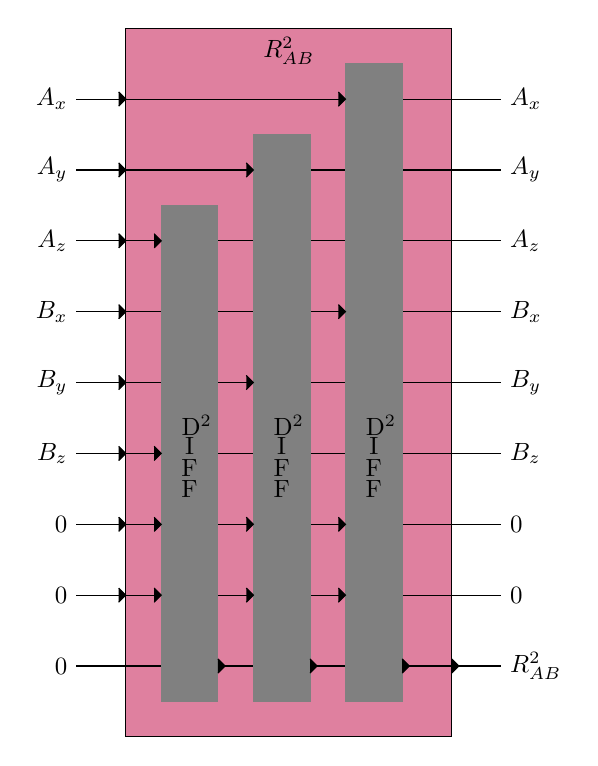
\begin{tikzpicture}[scale=.9, transform shape]
    \filldraw[fill=purple!50] (-1.3,9) rectangle (3.3,-1) ;
    \node[anchor=north] at (1,9) {$R_{AB}^2$};
    
    \node[rectangle,anchor=east] at (-2,8) {$\ket{A_x}$};
    \node[rectangle,anchor=east] at (-2,7) {$\ket{A_y}$};
    \node[rectangle,anchor=east] at (-2,6) {$\ket{A_z}$};
    \node[rectangle,anchor=east] at (-2,5) {$\ket{B_x}$};
    \node[rectangle,anchor=east] at (-2,4) {$\ket{B_y}$};
    \node[rectangle,anchor=east] at (-2,3) {$\ket{B_z}$};
    \node[rectangle,anchor=east] at (-2,2) {$\ket{0}$};
    \node[rectangle,anchor=east] at (-2,1) {$\ket{0}$};
    \node[rectangle,anchor=east] at (-2,0) {$\ket{0}$};

    \node[rectangle,anchor=west] at (4,8) {$\ket{A_x}$};
    \node[rectangle,anchor=west] at (4,7) {$\ket{A_y}$};
    \node[rectangle,anchor=west] at (4,6) {$\ket{A_z}$};
    \node[rectangle,anchor=west] at (4,5) {$\ket{B_x}$};
    \node[rectangle,anchor=west] at (4,4) {$\ket{B_y}$};
    \node[rectangle,anchor=west] at (4,3) {$\ket{B_z}$};
    \node[rectangle,anchor=west] at (4,2) {$\ket{0}$};
    \node[rectangle,anchor=west] at (4,1) {$\ket{0}$};
    \node[rectangle,anchor=west] at (4,0) {$\ket{R_{AB}^2}$};
    \foreach \y in {0,...,8}
        \draw (-2,\y) -- (4,\y) ;
    \foreach \y in {1,...,8}
        \filldraw[black] (-1.4,\y-.1) -- (-1.3,\y) -- (-1.4,\y+.1);
    \filldraw[black] (3.3,-.1) -- (3.4,0) -- (3.3,+.1);
    \foreach \x in {0,...,2}{
        \filldraw[gray] (-0.8+\x*1.3,6.5+\x) rectangle (0+\x*1.3,-.5);
        \filldraw[black] (\x*1.3,-.1) -- (\x*1.3+0.1,0) -- (\x*1.3,.1);
        \foreach \y in {1,2}{
            \filldraw[black] (\x*1.3-.9,\y-.1) -- (\x*1.3-0.8,\y) -- (\x*1.3-.9,.1+\y);
        }
        \foreach \y in {3+\x,6+\x}{
            \filldraw[black] (\x*1.3-.9,\y-.1) -- (\x*1.3-0.8,\y) -- (\x*1.3-.9,.1+\y);
        }
        \node[] at (\x*1.3-0.3,.5+2.9) {D$ ^2$}; 
        \node[] at (\x*1.3-0.4,.5+2.6) {I}; 
        \node[] at (\x*1.3-0.4,.5+2.3) {F}; 
        \node[] at (\x*1.3-0.4,.5+2) {F}; 
    }
\end{tikzpicture}
\caption{Circuits for calculating $\ket{a}\ket{b}\ket{acc}\to \ket{a}\ket{b}\ket{acc+(a-b)^2}$ and $\ket{A}\ket{B}\ket{0}\to \ket{A}\ket{B}\ket{R_{AB}^2}$}
\end{figure}
Using this circuit along with a constant addition of $\eta_{AB,ll'}$ and the use of an inverse square root circuit\cite{häner2018} we get a fixed point approximation of $\gamma_{AB,ll'}$. We can use this with a QFT fused multiply add operation to get the inner sum of the $E^\gamma$ term. There could potentially be a lot of pairs, however we can skip almost half with the following rewrite:
\begin{gather}
    \begin{split}
    E^\gamma&=\frac{1}{2}\sum_{A,B}\sum_{l\in A}\sum_{l'\in B} q_lq_{l'}\gamma_{AB,ll'}\\
        &=\sum_{A}\sum_{l\in A}\left[\sum_{l'\in A} q_lq_{l'}\gamma_{AA,ll'}+\sum_{B>A}\sum_{l'\in B} q_lq_{l'}\gamma_{AB,ll'}\right]
    \end{split}
\end{gather}
This rearrangement is also something they do in the xtb software.
Let us take take a brief look at the complexity of these quantum algorithms. 

\subsection{Complexity}
All these algorithms use $i = \lceil log_2(f) \rceil$ qubits to keep the fullerene IDs, where $f$ is the number of fullerenes in the isomer space $C_c$ that we are considering, thus $O(f^9)$. 

The first circuit uses 5 QFT fused multiplication addition circuits. Each with $O(b^{3})$\cite{perez2017} gates and no additional qubits, where $b$ is the number of bits used to encode the numbers. Thus if we have encoded an isomer space we need the two $\varGamma_0,\varGamma_1$ as well as the partial Mulliken charges for each atom $q_{A,0},q_{A,1}$ each using $b$ bits we will need to perform $10c$ multiplications, resulting in $10c\cdot O(b^3)=O(cb^3)$ gates, on $i + 2cb + 2b + 3b = O(cb+i)$ qubits. We can do trade-offs in circuit depth and amount of ancillary qubits by having multiple running sums e.g. in a binary tree pattern instead of immediately summing them all in the same register, resulting in a depth of $O(log_2(c)b^3)$. 

If we add in the sampling step we then have to run the state preparation circuit which adds $O(\log b)$ qubits and $O(b\log b)$ gates\cite{wang2020}, however that is not enough to change the asymptotic runtime further given $b<c$ in most cases we care about. 

If we want to say something about the number of samplings needed to have found a good candidate we have to assume a distribution for the energies in the isomer space. As a best guess we will assume they are evenly distributed between the highest and lowest energies $E^\Gamma_H$ and $E^\Gamma_L$. Then for a successful run of the algorithm the probability of sampling a given id is proportional to the energy $E_{id}^\Gamma$. Let us first find the exact proportionality.
\begin{equation}
    1=\int_{E^\Gamma_L}^{0}eC \,de=\int_{E^\Gamma_L}^{E^\Gamma_H}eC \,de
\end{equation}
If we solve for C
\begin{equation}
    C = -\frac{2}{{E^\Gamma_L}^2-{E^\Gamma_H}^2}
\end{equation}
Then the probability of sampling a fullerene with energy within $\delta$ of $E^\Gamma_L$ is 
\begin{equation}
    \begin{split}
        \int_{E^\Gamma_L}^{E^\Gamma_L+\delta}-\frac{2e}{{E^\Gamma_L}^2-{E^\Gamma_H}^2} \,de&=-\frac{2}{{E^\Gamma_L}^2-{E^\Gamma_H}^2}\int_{E^\Gamma_L}^{E^\Gamma_L+\delta}e \,de\\
        &=-\frac{2}{{E^\Gamma_L}^2-{E^\Gamma_H}^2}\left(\frac{(E^\Gamma_L+\delta)^2}{2}-\frac{(E^\Gamma_L)^2}{2}\right)\\
        &=-\frac{2}{{E^\Gamma_L}^2-{E^\Gamma_H}^2}\frac{(E^\Gamma_L+\delta)^2-(E^\Gamma_L)^2}{2}\\
        &=-\frac{2}{{E^\Gamma_L}^2-{E^\Gamma_H}^2}\frac{(E^\Gamma_L+\delta+E^\Gamma_L)(E^\Gamma_L+\delta-E^\Gamma_L)}{2}\\
        &=-\frac{2}{{E^\Gamma_L}^2-{E^\Gamma_H}^2}\frac{(2E^\Gamma_L+\delta)\delta}{2}\\
        &=-\frac{2E^\Gamma_L\delta+\delta^2}{{E^\Gamma_L}^2-{E^\Gamma_H}^2}
    \end{split}
    \label{eq:prob}
\end{equation}
This is only indirectly related to the size of the isomer space, as we might expect the gap between the highest and lowest energy in the isomer space scale with its size. 

For the second circuit we use $log_2(b)+log_2(c)+1$ control qubits and $2cb+2b+8cb+i$ for the rest giving a total on the order of $O(cb+i)$.
In terms of gates we use $c(2b+1)$ multiple controlled rotation gates, at most $log_2(b)+log_2(c)+1$ Hadamard gates, and $5c+1$ multiple controlled not gates. This gives a circuit depth on the order of $O(cb)$. 

The algorithm for calculating $E^\gamma$ uses $i+3cb+2cb+9b$ to hold the ids, positions, partial Mulliken charges and ancillaries. The 9 ancillaries are for the inverse square root approximation assuming 5 newton iterations. They are cleaned up afterwards, so the few we need for the rest of the algorithm can be taken from here. Thus we use $O(cb+i)$ qubits. 

In terms of gates we use 8 subtraction circuits and 3 multiplication circuits for each pair of atoms. For each pair of charges we do an addition by a constant the inverse square root and use 3 fused multiply add operations to add it to the running sum. For the inverse square root we will assume 5 iterations and the number of bits before the decimal point is equal to $b$. These assumptions make the complexity for the inverse square root $O(b^2)$ which is slightly worse than the actual complexity for a more reasonable number of bits before the decimal point, however it is still not the dominating factor. The subtraction circuits have similar complexity to the addition circuits already mentioned. This gives a total gate complexity of $c^2(8\cdot O(b^2)+3\cdot O(b^3)) + (2c)^2(O(b^2)+O(b^2)+3\cdot O(b^3))=O(c^2b^3)$

These complexities are not very impressive for a single computation, in which case we would get better results just running it classically. However if we have an isomer space $C_c$ with $f$ isomers we would have to run it on $n$ of them to have a probability of $\frac{n}{f}$ of having found the lowest energy isomer. Using the algorithm analysed in equation \ref{eq:prob} probability of having found a good candidate after $n$ samplings is only loosely dependent on $f$:
\begin{equation}
1-\left(1+\frac{2E^\Gamma_L\delta+\delta^2}{{E^\Gamma_L}^2-{E^\Gamma_H}^2}\right)^n
\end{equation}
Considering that $f$ is on the order of $O(c^9)$ for the $C_c$ space, that enables us to potentially run this on much larger isomer spaces and still have a high probability of getting some of the lowest energy candidates. This works only because we took care to sample in such a way that the probability of getting a specific candidate is proportional to its energy or, if we want to improve this result, how different it is energetically to a known high energy isomer. 

Aassuming a fixed $b$ the number of qubits used for each of these quantum algorithms scales with $O(c+i)$ and the circuit depth scales with $O(c)$ or $O(c^2)$. This is modest compared to the size of the isomer spaces we are feeding into them as a super position.

%\subsection{Cleaning up $\omega$}
%We would like to get rid of the $\ket{\omega}$ term in both algorithms to avoid having to post select.
%We can achieve this with amplitude amplification. 
%To do amplitude amplification we first need to define what a 'good' state is, in our case we know all good states have $\ket{0}_C\ket{1}_W$. 
%Second we need an oracle in terms of a unitary which flips the sign of the good state, i.e. reflecting the state around the bad state, this would be $I-2\ket{0}_C\bra{0}_C\ket{1}_W\bra{1}_W$, which can be easily implemented with controlled rotations. 
%We also need a circuit which would reflect around the initial state by flipping the sign of it, given that we have a circuit $U$ for preparing the initial state that would be $I-2U\ket{0}\bra{0}U^\dagger$.
%In our case the angle between the bad and initial states are $\theta_{DA} = arcsin(\frac{1}{2}\frac{E^\Gamma}{2^n}),\theta_{AA} = arcsin(\frac{1}{2^4}\frac{E^\Gamma}{2^{n4}})$ for the two algorithms. We have to do $\lfloor\frac{\pi}{4\theta}\rfloor$ repetitions to maximize the probability of measuring a good state.%Todo: fix every calculation and number in this. the propably all wrong 
%\subsection{Concentrating the probabilities on the best candidates}
%We now have a superposition where the probability of sampling a fullerene is proportional to the energy of that fullerene.
%But is that ideal? The energies might be quite close to each other in absolute terms.
%Therefore we would like to exaggerate the difference between them and then sample according to that difference.
%If we knew what the highest energy was we could just subtract that from every energy calculation thus getting probabilities proportional to how much lower an energy we are working with.
%Another option is if we expect the energies to be within $100(1-x)\%$ we could subtract $ex$ from every energy calculation where $e$ is the energy from a random fullerene in the isomer-space.
%This is of cause not as good but quite achievable. In both algorithms we can encode $ex$ in a register and then use a digital subtraction or do a QAA state preparation addition but with all the $R_y$ gates inverted, resulting in a counter-clockwise rotation, in effect subtracting $ex$.
%%Note: the following is dumb, we don't want to invert the probabilities! 
%If we expect the results from these shifted energy calculations to be in the interval $]0,1[$ we can exaggerate them further by taking the reciprocal. 
%\subsection{Discussion}
%From the asymptotic resource use the second algorithm is clearly superior, even if some of the multiplications and additions can be run in parallel in the first one. We do have a factor 8 lower chance of getting a useful state out, but this again does not change the asymptotics, as we can just repeat it. 
%QA-Amplification might be possible since we have a very clear "good" state in both algorithms. This would reduce the need for postselection and repetitions. Preparing the initial encoding of the isomer space seems less straight forwards in the second approach than in the first unfortunately. 
